\documentclass[thesis.tex]{subfiles}

\begin{document}

\chapter{Grundlagen}\label{chap:grundlagen}

\section{Aktuelle Alleinarbeitslösungen}\label{chap:alleinarbeit}

Im Arbeitsalltag treten immer wieder Situationen auf, die zur Gefährdung von Personen führen.
Diese Situationen ergeben sich aus den verschiedenen Arbeitsverfahren, Tätigkeiten, Werkstoffen sowie Umgebungen, die in allen Arbeitsbereichen unterschiedlich zur Geltung kommen.
Arbeit, die eine deutliche Gefährdung in diesen Faktoren aufweist, wird als \glqq Gefährliche Arbeit\grqq{} klassifiziert.
Beispiele dafür sind das Arbeiten in engen Räumen wie Silos oder Containern, Feuerarbeiten in brand- oder explosionsgefährdeten Bereichen oder in geschlossenen Räumen, Gleisarbeit während des Bahnbetriebes, Feuerwehr, Tunnelbau, Umgang mit besonders gefährlichen Stoffen, aber auch eine Dienstleistung an Personen zu verüben, die sich gegen diese tätlich wehren.
Letzteres kommt besonders bei der Polizei oder in sozialen Bereichen vor \cite[vgl.~S.~41 2.7.1]{Regel_100-001}.

In den meisten Fällen sollten gefährliche Arbeiten von mehreren Personen gemeinschaftlich ausgeführt werden.
Zur Vermeidung von Gefahren muss die Aufsichtspflicht durch eine zuverlässige, mit der Arbeit vertraute Person durchgeführt werden, die die gegenseitige Verständigung koordiniert, um die arbeitssichere Durchführung zu gewährleisten \cite[vgl.~§~8.1]{Vorschrift1_DGUV}.
In Ausnahmen kann es durch betriebliche Umständen notwendig sein, eine einzelne Person mit dieser Art von Arbeit zu betrauen. Dies ist grundsätzlich zulässig und kommt im Arbeitsalltag vielfach vor.
Alleinarbeit liegt laut DGUV vor, wenn eine Person allein, außerhalb von Ruf- und Sichtweite zu anderen Personen, Arbeiten ausführt \cite[S.~41~2.7.2]{Regel_100-001}.
Wird eine gefährliche Arbeit als Alleinarbeit vollzogen, muss ein Unternehmer über die allgemeinen Schutzmaßnahmen hinweg für ausreichend technische oder organisatorische Personenschutzmaßnahmen sorgen.
Zu diesen Maßnahmen zählen beispielsweise der Einsatz von Personen-Notsignal-Anlagen (PNA), ununterbrochene Kameraüberwachung, Kontrollgänge einer zweiten Person sowie kontinuierliche Meldungen durch Telefon- und Funksysteme \cite[vgl.~S.~43~2.7.2]{Regel_100-001}.
Dies soll sicherstellen, dass in einem Notfall der Alleinarbeiter so schnell wie möglich einen Notruf absetzten kann.
Die Notrufmöglichkeiten sind ein wichtiger Teil der Rettungskette.
Die Notwendigkeit verschiedenen Möglichkeiten zur Gefahrenminimierung werden durch die Gefährdungsstufen, Erstversorgungszeit und die Notfallwahrscheinlichkeit festgelegt \cite[vgl.~S.~13-18]{Regel_112-139}.

\begin{figure}[h]
    \centering
    \includegraphics[height=0.7\textwidth]{/Alleinarbeit_Maßnahmen.png}
    \caption{Mögliche Maßnahmen bei Alleinarbeit nach \cite[]{Information_212-139}}
    \label{fig:alleinarbeit_beurteilung}
\end{figure}

Wie in der \autoref{fig:alleinarbeit_beurteilung} ersichtlich wird, kann bei Alleinarbeit die Gefährdung in drei verschiedene Stufen eingeteilt werden.
Geringe Gefährdung heißt dabei, dass die allein arbeitende Person sich nach einem schädlichen Ereignis nur geringe Verletzungen zuziehen wird bzw. nur eine geringe akute Beeinträchtigung der Gesundheit verursacht wird.
Die Person bleibt also nach einem Unfall noch voll handlungsfähig.
Wie der Grafik zu entnehmen ist, ist dies der einfachste Fall.
Hier reicht eine Festnetzverbindung aus, um z.~B. den Notruf wählen zu können.
Die zweite Stufe ist die der erhöhten Gefährdung.
Bei dieser kann ein Alleinarbeiter erhebliche Verletzungen bzw. eine starke akute Beeinträchtigung der Gesundheit erleiden.
In diesem Fall bleibt die Person nach einem Notfall nur eingeschränkt handlungsfähig.
Bei einer hohen Wahrscheinlichkeit eines schädlichen Ereignisses muss diese Art von Tätigkeit sogar als kritische Gefährdung betrachtet werden.
In Bezug auf den Einsatz einer geeigneten Meldeeinrichtung dürfen jetzt keine stationären bzw. leitungsgebundenen Einrichtungen mehr benutzt werden.
Je nach Arbeit können hier aber Mobiltelefone, Sprechfunkgeräte, zeitgesteuerte Kontrollanrufe, durchgehende Kameraüberwachung oder PNAs zum Einsatz kommen.
Die letzte Stufe ist die kritische Gefährdung.
In der höchsten der drei Stufen können sich allein arbeitende Personen besonders schwere Verletzungen bzw. Beeinträchtigungen der Gesundheit zu ziehen.
Sie sind nach einer schädlichen Situation vollständig handlungsunfähig.
Bei dieser Stufe ist eingehend zu prüfen ob Alleinarbeit überhaupt zulässig ist.
Anderenfalls kann das Unternehmen an diesem Ort unter den gegebenen Umständen keine Alleinarbeit vollführen.
Hier kommen als Meldeeinrichtung nur noch die ständige Kameraüberwachung in Verbindung mit einem PNA infrage \cite[vgl.~S.~7-9]{Information_212-139}.

LKWs im Werksverkehr, Reinigungsfachkräfte und Taxifahrten während der Tagesschicht fallen dabei unter die geringe Stufe.
Gefahrguttransporte, Jugendhilfen und Dacharbeiten lassen sich in die zweite Kategorie einordnen.
Als kritische Gefährdung zählen Werttransporte, Aufzugmontage und -instandhaltungen und Taxifahrten bei Nacht.
Grundsätzlich ist diese Einteilung nur eine grobe Einordnung in die unterschiedlichen Stufen.
Bei jeder Arbeit muss eine individuelle Gefährdungsanalyse durchgeführt werden, da wie oben erwähnt, die Art der Tätigkeit, die Umgebung und andere Faktoren einen großen Einfluss auf die Sicherheit haben.
Gleiches gilt für den Einsatz der verschiedenen Meldeeinrichtungen in den Stufen.
Hier muss ebenfalls abgewägt werden, welche Einrichtung für den Einsatz ausreichend geeignet ist \cite[vgl.~S.~7-9]{Information_212-139}.

Um die Gefährdung einer Arbeit genau festlegen zu können, gibt es gemäß DGUV-Regel 112-139 \cite[]{Regel_112-139} die Bewertung der Arbeiten in verschiedene Schutzniveaus.
Dabei spielen die eben beschriebenen Gefährdungsstufen, die Zeit bis zu einer Erstversorgung und die Wahrscheinlichkeit eines Notfalls eine Rolle.
Mithilfe dieser Faktoren lässt sich ein Schutzniveau errechnen, welches für die Einteilung der Arbeiten genutzt wird.
Nach dieser Einteilung werden dann Maßnahmen festgelegt, um die Sicherheit zu erhöhen, die Notfallkette zu gewährleisten oder um ein Verbot von Alleinarbeit zu bestimmen.

Bei Betrachtung der einzelnen Meldeeinrichtungen fällt die PNA besonders auf, da diese als einzige ohne zusätzliche Maßnahmen in allen drei Stufen eingesetzt werden kann.
Geeignet ist auch das Mobiltelefon (bzw. Smartphone), da dieses Gerät sehr weit verbreitet ist und es bereits viele Menschen im Alltag verwenden.
Mit ihm können immerhin die geringe und teilweise die erhöhte Gefährdung gut abgedeckt werden.
Es eignet sich jedoch nicht für die kritische Stufe, da es bestimmte Hardware-Anforderungen, die in der Industrie benötigt werden, nicht erfüllt.
Darunter zählen der ausreichende Schutz vor Wasser, Staub, Chemikalien und rauem Umgang sowie der Gebrauch in sehr hohen oder niedrigen Temperaturen.
In dieser Gefährdungsstufe muss die Alarmauslösung zu jeder Zeit gewährleistet werden.
Dazu müssen die verwendeten Geräte einen hardwareseitigen, roten Alarmknopf besitzen.
Diese Anforderungen erfüllen handelsübliche Smartphones nicht.
Dafür können sie sehr einfach in den geringeren Stufen eingesetzt werden.
In diesem Fall kann sich der Einsatz einer Notfall-App anbieten.
Diese überträgt ein Notsignal an eine vorher festgelegte Stelle, um bei Bedarf die Rettungskräfte zu alarmieren.
Bei guter Programmierung kann die App den Einsatzkomfort des Smartphones in Notfallsituationen deutlich erhöhen und die Belastung auf den Arbeitenden reduzieren \cite[vgl.~S~.2-5]{FAQ-PNAuAPP}.

Die PNA kann jedoch in allen Gefährdungsbereichen eingesetzt werden und erfüllt auch die Industrieanforderungen.
Sie nutzt unter anderem die öffentlichen Mobilfunknetze, um eine dauerhafte Verbindung zu einer Empfangseinrichtung zu gewährleisten.
Durch die Hardware-Notruftaste, eine Lokalisierung über das \glqq Global Positioning System\grqq{} (GPS), Überwachung der Verbindung sowie des Gerätestatus und vorher definierten Alarmparametern, stellt sie die umfangreichste Lösung für Alleinarbeit dar.
Alarmparameter sind beispielsweise professionelle Alarmbearbeitung durch eine Notrufzentrale, wiederholte Alarmübertragung und Voralarme \cite[vgl.~S.~2-5]{FAQ-PNAuAPP}.
Alle Bauanforderungen und Funktionen die eine PNA erfüllen muss, sind in der DGUV-Regel 112-139 \cite[]{Regel_112-139} beschrieben.
Diese beruht auf der Norm "DIN VDE V 0825-11: Geräte- und Prüfanforderungen für Personen-Notsignal-Anlagen unter Nutzung öffentlicher Telekommunikationsnetze".
Die als Gegenstand dieser Arbeit vorgestellte Body-Cam ist in die Kategorie PNA einzuordnen.
Genauere Details der einzelnen Funktionen werden in \autoref{chap:funktionen} beschrieben.

\section{IST-Zustand Body-Cam}

\begin{figure}[h]
    \centering
    \subfloat[][]{
        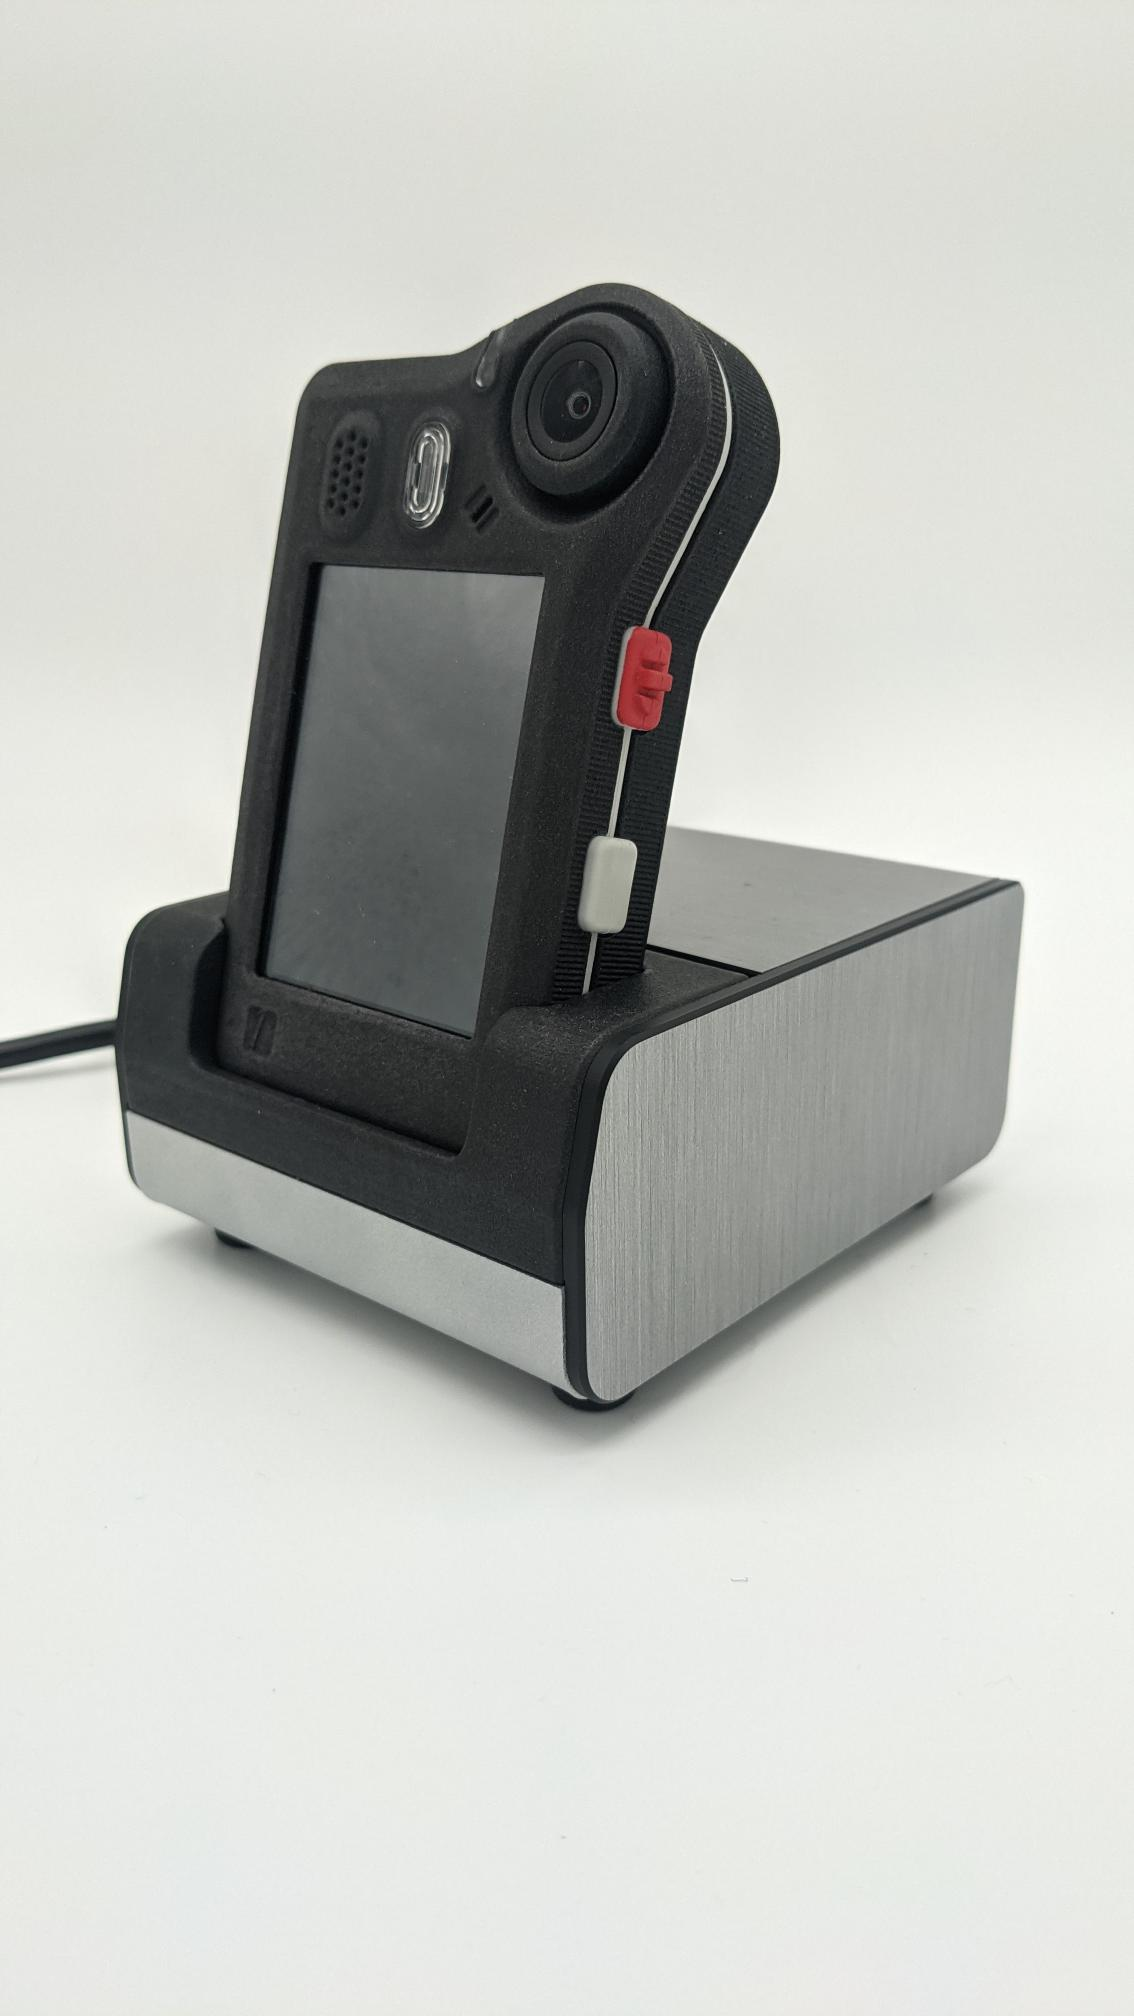
\includegraphics[height=0.50\textwidth]{/BC_side_dock.png}
        }
    \qquad
    \subfloat[][]{
        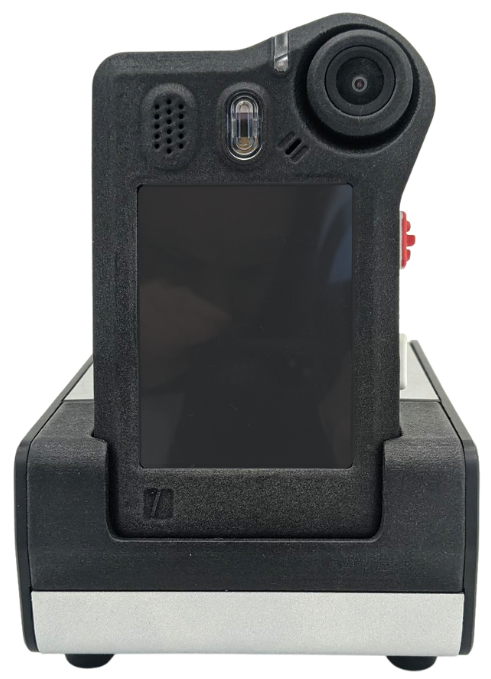
\includegraphics[height=0.50\textwidth]{/BC_front_dock.png}
        }
    \caption{Body-Cam in einer Dockingstation}
    \label{fig:BC_dock}
\end{figure}

Die Body-Cam ist das Hauptprodukt von NetCo und wurde 2016 entwickelt. Mittlerweile kommt sie europaweit erfolgreich zum Einsatz.
In erster Linie wurde sie zur Prävention und Deeskalation bei Konflikten entwickelt und kommt bei Polizeien, Ordnungsämtern, Verkehrsbetrieben und Sicherheitsdiensten zum Einsatz.
Hier vor allem zur Dokumentation von Einsätzen und zur rechtskonformen Beweissicherung und deren Gerichtsverwertbarkeit.

Die Body-Cam ist mit ihren Maßen von 102x62x25 mm kompakt gehalten und lässt sich daher gut während unterschiedlicher Arbeiten am Körper tragen ohne zu behindern.
Außerdem hat sie trotz der relativ geringen Größe ein 2,8 Zoll (ca. 7 cm) Farbdisplay mit integrierter Touchfunktion und einer Weitwinkelkamera. Dadurch lassen sich sehr einfach alle Statusinformationen ablesen und es können sowohl Textnachrichten als auch der aktuelle Videostream angezeigt werden.
Der Touchscreen lässt sich auch problemlos mit Handschuhen bedienen, was gerade im Einsatz sehr wichtig ist.
Sie kann in einem Temperaturbereich von -20 Grad bis + 50 Grad Celsius betrieben werden.
Zusätzlich besitzt sie die Schutzklasse IP 65 und ist damit dicht gegen Staub und geschützt gegen Strahlwasser \cite[S.44]{Elektro_Baugruppen}.
Die Kamera zur Videoaufzeichnung hat ein 160 Grad Weitwinkel-Objektiv und verfügt über eine hohe Lichtstärke.
Damit kann sie die Situation des Trägers in einem großen Bereich erfassen und auch Aufnahmen bei schlechter Beleuchtung oder bei Dämmerung gut darstellen.
Der Akku versorgt die Body-Cam, sowie eine integrierte helle LED-Lampe mit Strom.
Die Kapazität der Batterie beträgt dabei 5.000 mAh.
Dieser große Akku ist notwendig, um eine Versorgung über eine ganze Schicht, also über 8 Stunden, zu gewährleisten.
Die Aufladung der Batterie erfolgt dabei über die zu der Body-Cam entwickelten Docking-Station.
Diese dient gleichzeitig zum Aufladen ein oder mehrerer Kameras, sowie zur Übertragung aller auf dem internen Speicher befindlichen Aufnahmen an ein zentrales System.
Die Body-Cam ist ebenfalls mit WLAN und Bluetooth ausgestattet.
WLAN kann in bestimmten Umgebungen die Mobilfunkverbindung ersetzten.
Beim Einsatz in Zügen der Deutschen Bahn lässt sich beispielsweise das im Zug integrierte WLAN nutzen, um bei der Zugfahrt unabhängig vom ständig wechselten Mobilfunknetz zu sein.
In Verbindung mit Geräten anderer Hersteller, wie z.B. einem Bluetooth-fähigem Waffenholster, kann die Body-Cam über Bluetooth mit diesem gekoppelt werden.
Hierdurch kann automatisch eine Aufnahme gestartet werden, wenn die Waffe aus dem Holster gezogen wird.
[vgl. \autoref{anhang:datenblatt}]

\begin{figure}[h]
    \centering
    \subfloat[][]{
        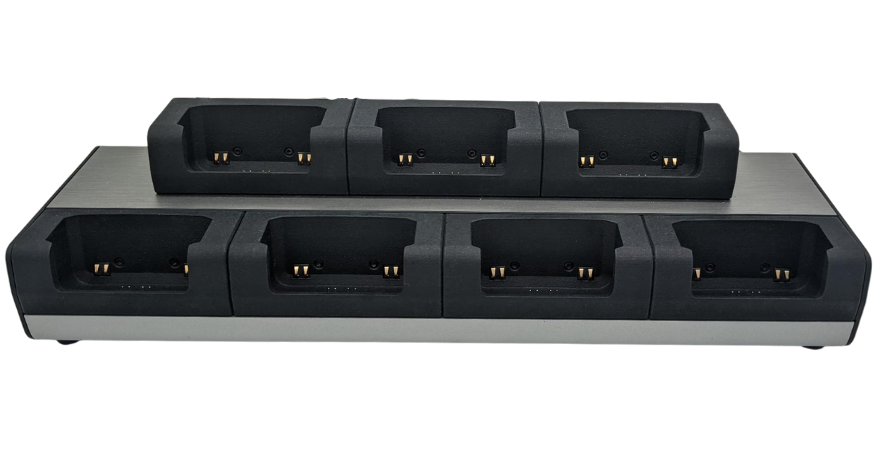
\includegraphics[width=0.45\textwidth]{/BC_docking_7_empty.png}
        }
    \qquad
    \subfloat[][]{
        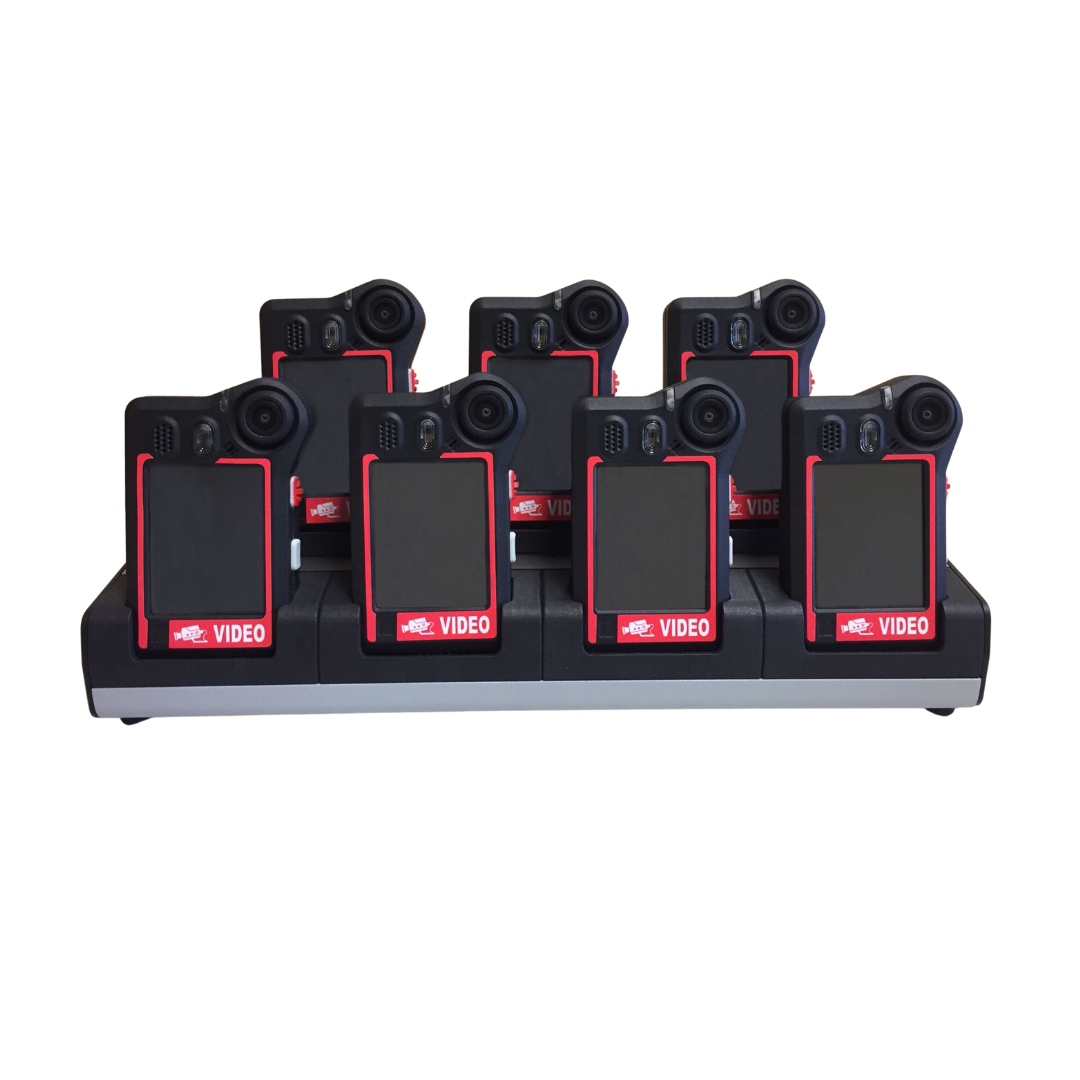
\includegraphics[width=0.45\textwidth]{/BC_docking_7_full.png}
        }
    \caption{Dockingstation mit der sieben Body-Cams gleichzeitig verwaltet werden können}
    \label{fig:BC_docking_7}
\end{figure}

Die NetCo Body-Cam wird grundsätzlich in zwei Versionen angeboten.
In der Record-Version wird die Aufnahme auf dem Gerät gespeichert und nach dem Einsatz automatisch über eine Docking-Station in das zentrale System überspielt.
Mit der 128 GB großen microSD-Karte lassen sich damit bis zu 17 Stunden Aufnahmezeit erreichen.
Die Aufnahmen werden dabei mit AES 256 Bit verschlüsselt.
Außerdem ist auch eine Voraufzeichnungsdauer von bis zu 2 Minuten möglich.
Die Voraufzeichnung findet dabei in einer Schleife statt und wird erst nach Bestätigung der Aufnahmetaste, der Aufnahme vorangestellt.
Dies dient zur Sicherstellung des Datenschutzes und hat zugleich den Vorteil, dass der Träger der Body-Cam in Gefahrensituationen erst handeln und dann die Aufnahmetaste drücken kann ohne, dass dabei Informationen verloren gehen.

In der Connect-Version erfolgt die unmittelbare Übertragung über ein gesichertes VPN an das zentrale System.
Dabei hat die Kamera eine 4G LTE Verbindung und kann die Aufnahmen nach Beendigung direkt an die zuständige Dienststelle übermitteln.
Dies ist beispielsweise in Situationen wichtig in denen zu Befürchten ist, dass die Herausgabe der Kamera mit Gewalt erzwungen wird.
Hier kann im Zweifel die Kamera herausgegeben werden, um eine weitere Eskalation zu vermeiden, ohne dass dabei Aufnahmematerial verloren geht.
Mit dem übertragenden Material kann dann umgehend eine Fahndung und Unterstützung eingeleitet werden.
% Beide Systemvarianten decken die Zielstellungen Prävention, Deeskalation und Dokumentation zuverlässig ab.

\section{Erweiterung der Body-Cam mit dem Alleinarbeits-Modus}

Durch die, im vorherigen Kapitel beschriebenen, umfassenden Einsatzmöglichkeiten und Funktionen, bringt die Body-Cam bereits sehr viele Eigenschaften mit, die sie als ein PNA für Alleinarbeit nach DGUV Regel 112-139 \cite[]{Regel_112-139} qualifiziert.
So besitzt die Body-Cam beispielsweise eine ausreichende Schutzklasse, ist mit Mobilfunk, WLAN sowie Bluetooth ausgestattet, kann bei sehr hohen und niedrigen Temperaturen betrieben werden und lässt sich einfach und zuverlässig in schwierigen Situation bedienen.
Außerdem bringt sie weitere Eigenschaften mit, die für ein PNA nicht direkt gefordert sind, aber die für die Alleinarbeit nützlich sind.
Hierbei ist z.B. die Kamera zu nennen mit der eine dauerhafte Überwachung durch einen Videostream möglich ist, sowie das vergleichsweise große Display, welches einen guten Überblick über alle Statuswerte verschafft.

Es gibt jedoch auch Hardwarekomponenten und Software die nachgerüstet werden müssen, um einen vollständigen Einsatz als PNA zu gewährleisten.
Einer der wichtigsten Eigenschaften ist das Auslösen eines Alarms.
Dieser soll in Gefahrensituationen einfach durch einen hardwareseitigen roten Knopf zuverlässig ausgelöst werden können.
Der rote Knopf ist bereits in der Body-Cam als Aufnahmeknopf verbaut und muss für die Lone-Worker Version nur mit der entsprechenden Alarmfunktion verknüpft werden.
Als Zweites muss noch ein Lagesensor nachgerüstet werden.
Dieser Sensor soll die Lage des Lone-Worker kontinuierlich überwachen und feststellen, wenn sich diese plötzlich ändert.
Das wird genutzt, um festzustellen, ob der Lone-Worker beispielsweise ohnmächtig in sich zusammengebrochen ist und damit handlungsunfähig ist.
Bei Eintreten dieses Ereignisses wird erst ein Voralarm ausgelöst, diesen kann der Träger bei Falschmeldung abstellen.
Anschließend wird ein richtiger Alarm an das Überwachungszentrum gesendet.
Dieser informiert, dass der Lone-Worker möglicherweise verunglückt und handlungsunfähig ist.
%% wie Ohnmächtig??

Die für den Einsatz als PNA benötigte Softwarefunktionen, werden durch den Lone-Worker-Modus repräsentiert.
Dieser ist Hauptbestandteil dieser Arbeit und wird in den folgenden Kapiteln beschrieben, designt und als Prototyp mit seiner Grundfunktionalität implementiert.
Grundsätzlich ist dieser dafür zuständig eine Verbindung zu einem Überwachungszentrum herzustellen und dauerhaft zu halten oder bei Bedarf umgehend wieder herzustellen.
Er übernimmt die Kommunikation zwischen Überwachungszentrum und Body-Cam mithilfe eines eigenen Protokolls.
Der Modus verwaltet alle Alarme, Voralarme und Alarmwiederholungen sowie die Statuswerte des Geräts.
Über die verschiedenen Schnittstellen zur Body-Cam, kann er dem Überwachungszentrum Geräteinformationen, Standorte, Video- und Audiostreams sowie einen Sprachkanal ununterbrochen zur Verfügung stellen.
Audio- und Videodaten sowie Standortinformationen werden dabei bereits durch Kamera, Mikrofon und GPS erfasst und müssen in die neue Funktion eingebunden werden.
Der Lone-Worker-Modus erweitert also die bestehenden Funktionen der Body-Cam zur Prävention, Deeskalation und Protokollierung um eine Möglichkeit sie als PNA für Alleinarbeit zuverlässig einzusetzen.

\section{Komponentenbeschreibung des Gesamtsystems}
% hier noch ne Graphik einfpügen die das zusammenspiel der Komponenten zeigt
Das Gesamtsystem setzt sich hauptsächlich zusammen aus der Body-Cam als Clientgerät, dem „Lone-Worker“
als Träger der Body-Cam sowie einem Überwachungszentrum als Server mit einem oder mehreren Operatoren.
Außerdem ist das Zentrum mit offiziellen Notrufstationen verbunden, um eine schnelle Rettung und Versorgung der Lone-Worker zu gewährleisten.

Der in sich in Alleinarbeit befindliche Arbeitende wird Lone-Worker genannt.
Er verrichtet die im \autoref{chap:alleinarbeit} genannte gefährliche Arbeit.
Um dies allein mit einer angemessenen Sicherheit tun zu können, wird er bei seiner Arbeit dauerhaft überwacht.
Zu diesem Zweck trägt er am Oberkörper die Body-Cam.
Die Body-Cam ist ein Embedded-Gerät, welches unter anderem eine Weitwinkelkamera zur Videoaufzeichnung sowie ein großes Display zur Bedienung hat.
Durch die Platzierung am Oberkörper des Trägers kann eine gute Sicht aus Perspektive einer Person gewährleistet werden.
Die Träger der Body-Cam schaltet zu Beginn seiner Arbeit das Gerät ein.
Dieses verbindet sich dann über z.B. das öffentliche Mobilfunknetz mit dem hinterlegten Überwachungszentrum.

Damit der Lone-Worker seine Arbeit aufnehmen kann, muss er den Lone-Worker-Modus an der Body-Cam einschalten.
Je nach Gefahreneinstufung muss diese Aktivierung durch einen Operator im Überwachungszentrum bestätigt werden.
Im aktivierten Lone-Worker-Modus kann sich der Alleinarbeiter auf eine durchgehende Verbindung verlassen.
Bei Störung der ununterbrochenen Kommunikation zum Überwachungszentrum wird der Arbeiter über die Body-Cam informiert.

Im Gefahrenfall kann der Lone-Worker einen Alarm auslösen, beispielsweise durch Betätigen des roten Knopfes oder automatisch durch den Lagealarm.
Dieser wird an das Überwachungszentrum übermittelt.
Dort wird der Alarm entweder direkt zu einer Notrufzentrale, mit allen verfügbaren Informationen, weitergeleitet oder zum Operator durchgestellt.
Der Operator nimmt dann umgehend Kontakt zum Lone-Worker auf.
Dies geschieht durch den Zwei-Wege-Audiokanal und durch die von der Body-Cam zur Verfügung gestellten Livestreams.
Bei Bedarf kann der Operator alle nötigen Schritte zur Rettung des Alleinarbeiters einleiten.

Das Überwachungszentrum dient als Leitstelle, zu welchem sich mehrere Geräte verbinden können.
Je nach zur Verfügung stehenden Kapazitäten (Operatoren) können strengere Überwachungen mit eingeschaltetem Lone-Worker-Modus durchgeführt werden.
Den Aufbau und Abbau von Verbindungen sowie das Anfordern und Darstellen von Informationen über die einzelnen Body-Cams wird
durch einen Automatismus realisiert.

% \section{Use-Cases}
\section{Anforderungen des Gesamtsystems}
Die Anforderungen die an das neue Lone-Worker Feature gestellt werden, ergeben sich durch verschiedene DGUV-Normen sowie zusätzliche Unternehmensanforderungen.
Folgenden Bestimmungen richten sich dabei an das Gesamtsystem des Lone-Worker Feature und sind keine Anforderungen an den praktischen Teil dieser Arbeit.
Der implementierte Prototyp legt einen Grundbaustein für die spätere Umsetzung aller Funktionalitäten des Lone-Worker-Modus.

Die Body-Cam sollte einen Schutz gegen versehentliche Aktivierung des Lone-Worker-Modus besitzen.
Dies lässt sich zum Beispiel wie folgt realisieren:
\begin{itemize}
    \item Die Aktivierung eines Voralarms, der ohne Konsequenzen abgebrochen werden kann.
    \item Ein spezielles Design des Aktivierungstasters. Hier kann beispielsweise ein versenkter Taster benutzt werden für den mehr Kraft zur Aktivierung benötigt wird.
    \item Die Dauer des Tastendrucks zur Aktivierung des Modus kann erhöht werden, sollte jedoch im Bereich von wenigen Sekunden sein.
\end{itemize}

Es sollte die Möglichkeit für eine Zweiwege-Audio-Verbindung zwischen Client und Server bestehen.
Dies schafft für den Lone-Worker die Gelegenheit Kommentare der überwachenden Person zu hören und auf diese zu antworten.
Außerdem kann der Lone-Worker nach mündlicher Aufforderung eine Aktion bestätigen oder Informationen über den Einsatzfortschritt geben.

Nach einer erfolgreichen Authentifizierung soll das Überwachungszentrum Fernzugriff zum Lone-Worker bekommen.
Dies soll folgende Optionen ermöglichen:
\begin{itemize}
    \item Abruf von Audio- und Videostreams sowie Standortdaten.
    \item Abruf von auf dem Gerät gespeicherten Mediendateien (Datengröße kann für LTE ggf. zu groß sein).
    \item Abfrage und setzten von Geräteparametern.
    \item Lesen des Gerätestatus
    \item Übertragung von neuer Firmware
\end{itemize}

Einige dieser Optionen, wie das Setzen von Geräteparametern oder ein Update der Firmware sollten nur bei ausgeschaltetem Lone-Worker-Modus und nach Bestätigung des Lone-Worker möglich sein.

Der Lone-Worker soll zu jeder Zeit die Möglichkeit haben Informationen über die Stärke des Netzwerksignals und den Batteriestatus am Gerät zu sehen. % siehe Abbildung Schema??
Hierfür soll der aktuelle Signalpegel und Batteriezustand auf dem Display zu sehen sein sowie ein haptisches, akustisches oder visuelles Feedback bekommen, wenn keine Verbindung verfügbar ist oder der Batteriestand in einen kritischen Bereich fällt.
Dem Überwachungszentrum sollen diese Informationen, sowie die Benachrichtigung bei kritischem Batteriezustand ebenfalls zur Verfügung stehen.

Dem Träger der Body-Cam soll die Gelegenheit haben einen \glqq Timer\grqq{} einzustellen.
Dieser dient dazu die Alarmfunktion temporär abzustellen und ist vor allem sinnvoll, wenn es zu einer erwartenden Einschränkung des Kommunikationsnetzes kommt.
Dies tritt beispielsweise auf, wenn sich der Lone-Worker in einen Fahrstuhl begibt.
In dem Fall kann der Träger ein Aussetzen der Verbindung in der Body-Cam vermerken.
In dieser Zeit wird bei Verbindungsverlust kein Alarm auf beiden Seiten der Kommunikation ausgelöst.
Das Überwachungszentrum wird über das Einschalten dieser Funktion informiert.
Wenn nach Ablauf der Zeit keine Verbindung hergestellt werden kann, gehen beide Parteien in den Alarmzustand über.
Der Lone-Worker hat die Möglichkeit den Timer vor Ablauf der Zeit zu deaktivieren und damit wieder in die normale Funktionsweise des Lone-Worker-Modus überzugehen.

Die Body-Cam soll dem Zentrum auf Anfrage die aktuelle Position oder eine Liste der letzten 50 bekannten Positionen übermitteln.
Dies wird vor allem dafür genutzt das Konfigurieren und Überwachen von \glqq Geo-Fences\grqq{} zu ermöglichen.
Damit können Ein- und Austreten aus bestimmten Bereichen überwacht werden und dem Überwachungszentrum automatische Benachrichtigungen
über diese Vorgänge gemacht werden.
Außerdem können auf der Body-Cam bestimmte Reaktionen konfiguriert werden die beim Betreten oder Verlassen von \glqq Geo-Fences\grqq{}-Gebieten aktiv werden.
Zum Beispiel lassen sich damit folgende Szenarien bei Ein- oder Austritt abbilden:
\begin{itemize}
    \item Aktivierung oder Deaktivierung des Lone-Worker-Modus.
    \item Automatische Übertragung des Audio- und Videostreams.
    \item Warnung des Lone-Worker durch ein konfigurierbares Feedback, vor dem Betreten eines besonderen Gefahrengebiets.
\end{itemize}

Das Überwachungszentrum soll die Möglichkeit haben, Statistiken über die einzelnen Geräte anfertigen zu können.
Dafür müssen alle Aktivierungsmeldungen, Alarme, einschließlich Fehlalarme erfasst werden.
Ebenfalls soll die Verfügbarkeit des Mobilfunknetzes aufgezeichnet werden.
Diese Informationen müssen von der Body-Cam bereitgestellt werden und sind vom Zentrum zu erfassen.
Außerdem soll die Body-Cam alle Events dokumentieren und auf ihrer SD-Karte speichern.
Darunter zählen die oben beschriebenen Auskünfte sowie alle Gerätestatusinformationen wie beispielsweise Batteriestatus
oder Speicherplatz, GPS-Standorte, Änderungen in der Konfiguration, Aktivierung und Deaktivierung des Lone-Worker-Modus
sowie des temporären „Timer“-Modus, Anfragen und Antworten von und an das MC und Softwareinformationen.

Die Body-Cam soll dem Lone-Worker ein haptisches, akustisches und visuelles Feedback geben können.
Dies kann in Form eines Voralarms sein, wie vorhergehend beim Aktivieren des Lone-Worker-Modus beschrieben oder beim Auslösen eines Alarms, um die Aufmerksamkeit des Lone-Worker zu erhalten.
Außerdem kann dadurch das Überwachungszentrum dem Lone-Worker durch ein haptisches Feedback einen \glqq Stillen\grqq{}-Alarm senden.
Weiterhin soll das Display der Body-Cam für visuelles Feedback sowie das Anzeigen von Textnachrichten genutzt werden.
Der Träger kann durch auf dem Display eingeblendete Optionen, die Fragen eines Operators beantworten.
Die verschiedenen Antwortmöglichkeiten sind vorher vom Operator festzulegen.

Die Body-Cam soll die Möglichkeit bieten die Konfigurationsmöglichkeiten einzuschränken, um ungewollte oder unbefugte Änderungen zu verhindern.
Dies dient in erster Linie der Sicherheit des Trägers und soll einen einfachen und schnellen Einsatz gewährleisten.
So können die Geräte vorher durch ein Unternehmen oder eine Abteilung konfiguriert und anschließend an die einzelnen Lone-Worker ausgeteilt werden.

\subfilebib % Makes bibliography available when compiling as subfile
\end{document}